\section{Soluții actuale}

Pentru jucătorii care doresc o anumită doză de adrenalină sau care preferă partide mai rapide de regulă se folosesc de un anumit ceas, fie el analog sau digital, în cadrul jocului de șah. Adăugând timpul ca o resursă jocul poate deveni mai interesant (sau frustrant) și stimulant pentru creier. Conform izvoarelor ceasurile au început să fie folosite în mediul profesionist începând din secolul XIX, un exemplu fiind „Turneul internațional de șah din Londra” (1883) \cite{bcm1883}. Ceasurile din această perioadă erau simpliste, oferind jucătorilor posibilitatea de a-și aloca un buget de timp, comuta între ture și cel mult de a fi avertizați de ultimele minute rămase prin intermediul unui „fanion” gravat pe cadran.

Totuși, lipsa preciziei a ceasurilor analogice și a altor funcționalități a determinat dezvoltarea dispozitivelor digitale programabile care ar fi oferit o mai bună precizie și o sporită flexiblilatate în configurarea timpului de joc (cum ar fi bonusul Fischer care reprezintă un interval de timp acordat fiecărui jucător după o mutare). Un prim exemplu\footnote{Unele surse vorbesc de un anumit Bruce Cheney care ar fi elaborat primul ceas digital în 1973, însă aceată afirmație nu a put fi confirmată.} îl constituie ceasul „Micromate-180” apărut în 1979 având la bază cercetarea efectuată de Joseph Meshi \cite{chess_life1992}.\\

\subsection{Digital Game Technology}
La ora actuală cea mai populară soluție este cea oferită de către compania DGT ce se prezintă ca o gamă largă de ceasuri lansate cu diferite scopuri în minte. Astfel, întălnim cele făcute cu scop competitiv oficial (cum ar fi modelul DGT 3000 folosit în această lucrare), pentru amatori și cele pentru persoanele cu dizabilități. Oferta celor de la DGT este cu atât mai atractivă dacă luăm in considerare faptul ca unele modele sunt compatibile cu seria lor de table de șah inteligente (table care memorează mișcările executate și care pot fi conectate la calculatoare personale) prin conectarea acestor printr-un model propriu de cablu (având la amblee capete conectori de tip Jack 3.5 mm) sau prin Bluetooth. Această conexiune se realizează automat cu ajutorul aplicației „Fritz” care vine împachetată cu tabla. Pentru mai multe detalii a se consulta manualul \cite{dgt_eboard_manual}.

\subsection{Picochess}
Proiect inițiat de Jean-Francois Romang cu scopul de a conecta o tablă intelgentă DGT la o placă de tip Raspberry Pi, acesta oferă utilizatorului de juca partide de șah folosind diferite \textit{chess engines} cum ar fi Stockfish, cronometra timpul și salva meciurile, toate acestea fiind posibile datorită plăcii menționate. Așa populară a devenit soluția oferită într-un cât incepând din anul 2016 DGT a lansat pe piață modelul DGTPi care integrează proiectul PicoChess \cite{pico_chess_overview}. Proiectul se află într-un \textit{repository} de Github\footnote{https://github.com/jromang/picochess} iar dacă l-am clona și rula comanda git log --reverse am observa că acesta își are originea din 30 iulie 2014\footnote{Dacă ar fi să fim riguroși atunci va trebui să considerăm data inițială drept 4 iulie 2011 odată cu următoarea discuție de pe forum: https://hiarcs.net/forums/viewtopic.php?t=5046}. Datorită naturii \textit{open source} a soluției și a implementării interfeței în Python, acesta este ușor de preluat și extins dacă există intenția.
\begin{figure}[H]
	\centering
	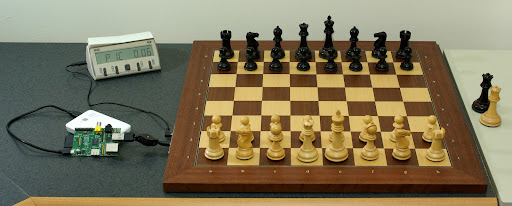
\includegraphics[width=0.7\textwidth]{img/picochess_setup.jpg}
	\caption{Folosind un ceas DGT 3000 împreună cu Picochess}
\end{figure}